\paragraph{}This chapter will explain the methodology and requirements for the \ac{SLAM} tuning module, developed for \ac{RUSTLE}. For each implemented tuning technique, a high level overview of its architecture is provided. Test settings, including test algorithms and dataset choices, are also justified.

\begin{figure}[h]
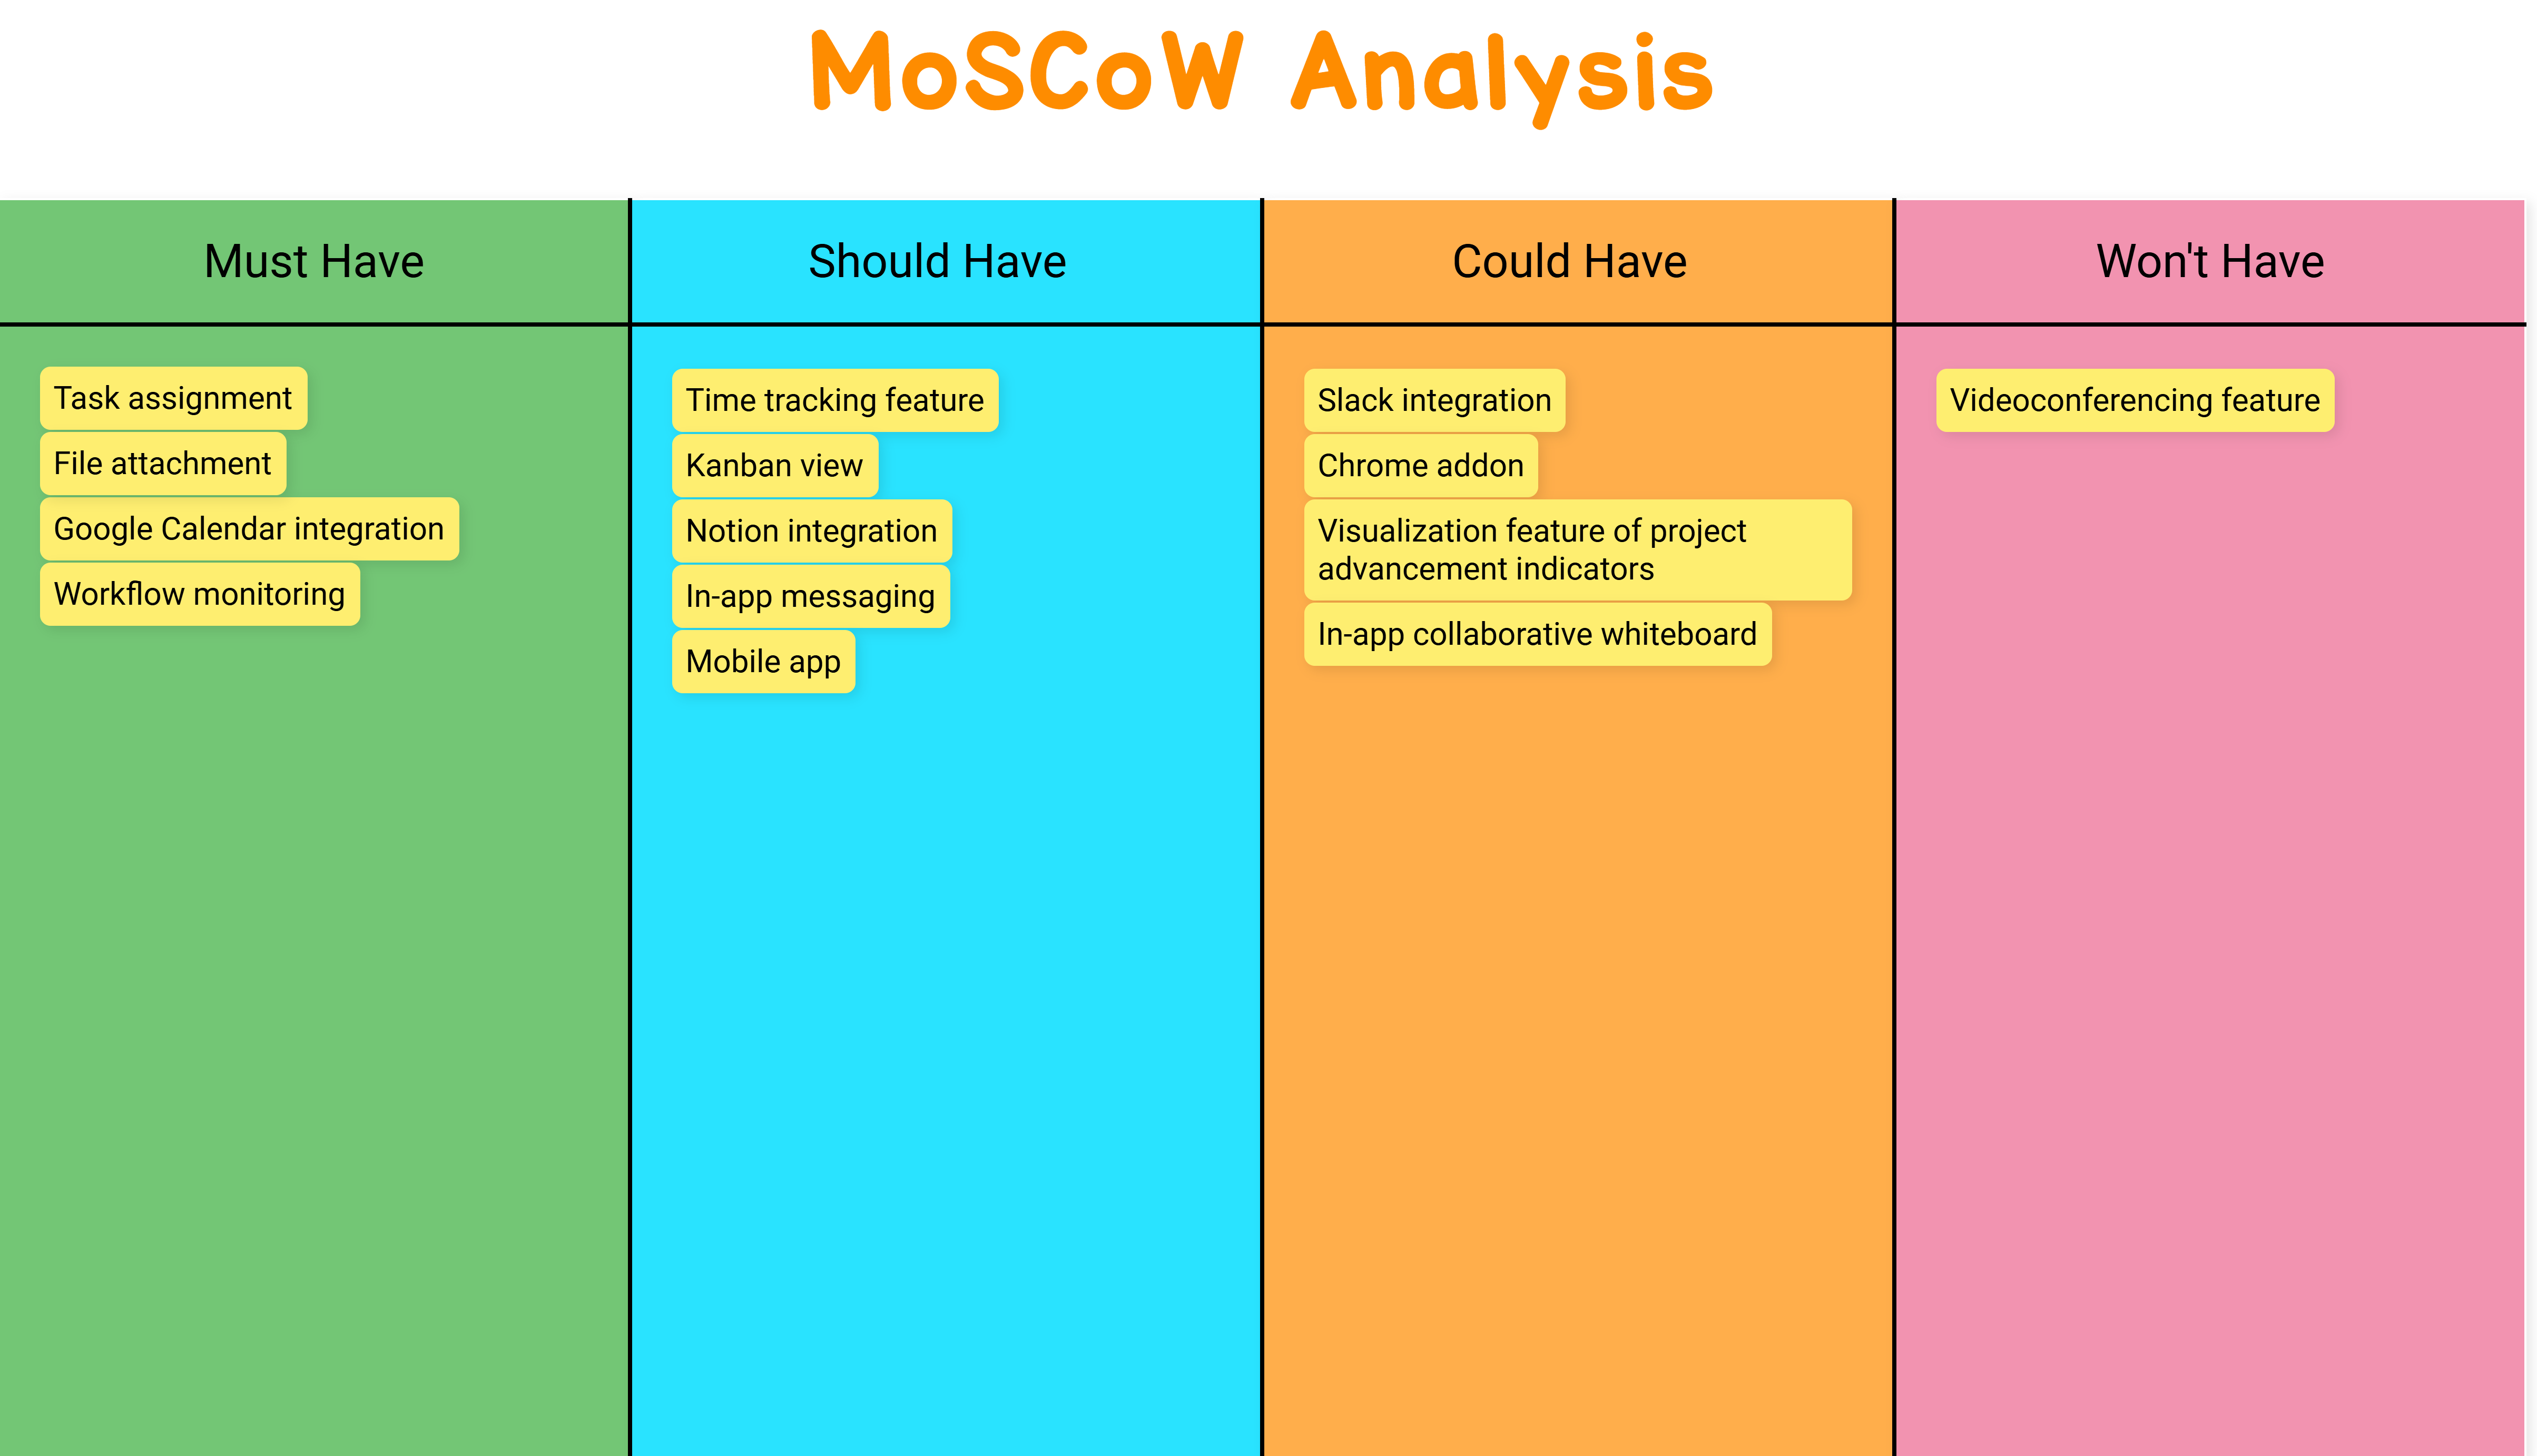
\includegraphics[width=0.85\linewidth]{images/moscow.png}
\end{figure}

\section{\ac{RUSTLE}}

\paragraph{}\ac{RUSTLE} is a command line application, written in Rust, which is designed to simplify the evaluation of SLAM algorithms in mobile robotics.
Its main objective is to provide a simple, stream-lined and reproducible way to run and compare SLAM algorithms. It tracks not only trajectory accuracy(APE or RPE), but also runtime, CPU load and memory usage, offering a more complete assessment of the algorithm's performance.

\paragraph{}At its core, RUSTLE takes three main inputs: a dataset in rosbag format, the SLAM algorithm's parameters in yaml format, and the algorithms themselves as docker images. The reason for using Docker is for reliably reproducing the algorithms across many different platforms and environments.
During execution, the odometry data is streamed into the database(Surrealdb), which, after conclusion, is used to calculate trajectory errors such as the APE and the RPE, using EVO.

\paragraph{}Algorithm executions are run as tests. Each test's configuration is passes as an YAML file, and contains: its name, number of workers, number of iterations, list of algorithms, dataset on which to execute these algorithms and the test type. Additionally, some additional fields might be required, depending on the type of test one wants to execute.

\paragraph{}As for language choice, Rust was chosen mostly due to simplicity of development and the ease with which one can write highly performant code. Other languages, such as c++ and python, also have libraries for working with Docker and ROS, as well as libraries for database hosting. The difference with Rust in this regard is that to use these libraries it is only needed to include them as dependencies, and use them in the codebase, as the download, compilation and linking of these libraries is all automatically handled by Rust's build tool, cargo. As for performance, Rust is known for its compile-time enforced memory safety(at the cost of some control over memory), as well as built in type system guarantees, which prevent common multithreaded issues like data races.

\section{Development}
\paragraph{}Development follows an incremental approach, focusing on small incremental features, well thought and tested. Each big feature, such as random search tuning, is divided into smaller "implementable" sub-features. The reason for this is to make it easier to reason about how to implement the feature, as well as, during development, to make it easier to test each sub-feature.

\section{Functional requirements}

\begin{itemize}
	\item allow the user to specify which tuning method, algorithm and dataset, and also the parameters to optimize using a yaml configuration file.
	\item For grid and random search, for any tuned parameters in the configuration file, the general pattern should be either a single value or an array of various values. For numerical parameters(integers or real numbers), a third option should be available: a linearly spaced vector, and that vector is specified through a 3 element array whose elements are [start, step, number\_of\_elements].
	\item Other settings, such as the budget or the cooling factor in the simulated annealing method, should have default values
	\item a budget parameter(B) should be either a maximum number of configurations to run or maximum alloted time. These should be represented by the keys \textbf{max\_iter} and \textbf{max\_time} in the configuration file.
	\item tuning a SLAM algorithm's parameters is classified as a test, for easier integration in the existing RUSTLE's architecture.
	\item when running a tuning test, all tested parameter combinations should have their respective metrics stored together, for later processing
	\item when running a tuning test, all tuning settings should be stored as well, for later processing and examination
	\item for overall testing and comparison of different tuning strategies, there should be a command to run a set of tuning algorithms and produce appropriate metrics which later could be displayed as a table or graph.
	\item The tuning module should run different configurations concurrently, when possible.
\end{itemize}

\section{Non Functional requirements}

\begin{itemize}
	\item The tuning module should be future proof, allowing for the easy addition of other tuning algorithms into the software.
	\item 
\end{itemize}

\section{Testing}

\subsection{Metrics}

\subsection{Algorithms}

\subsection{Datasets}